% Beamer version of the "Sorting Networks of Logarithmic Depth" slide deck.
% Retains the original deck sequence, palette and diagrams with claims aligned to the report.
% Diagrams are drawn in TikZ using the HTML deck's pixel coordinates (1920 x 1080 canvas = 16cm x 9cm).
% Revised against the integrated report. Compile with: pdflatex slides.tex
% The existing palette, typography and TikZ illustrations are retained; bound comparisons are added.
% Speaker notes are included with \note{}; to show them, add \setbeameroption{show notes on second screen=right}.
\documentclass[aspectratio=169,9pt,xcolor=table]{beamer}

\usepackage[T1]{fontenc}
\usepackage{lmodern}
\usepackage[sfdefault]{plex-sans}
\usepackage[lining]{ebgaramond}
\usefonttheme[onlymath]{serif}
\usepackage{amsmath,amssymb}
\usepackage{booktabs}
\usepackage{tikz}
\usetikzlibrary{shapes.arrows,arrows.meta}
\usepackage[most]{tcolorbox}

% ---------- palette ----------
\definecolor{navy}{HTML}{14213D}
\definecolor{ink}{HTML}{3A4659}
\definecolor{paper}{HTML}{F7F5EF}
\definecolor{paperalt}{HTML}{ECE8DD}
\definecolor{rust}{HTML}{A63D26}
\definecolor{rustlight}{HTML}{E9A58F}
\definecolor{steel}{HTML}{2F5F8A}
\definecolor{mist}{HTML}{C9D3E0}
\definecolor{muted}{HTML}{5F6B7D}
\definecolor{hl}{HTML}{FBE9E3}
\definecolor{softrust}{HTML}{F2D9D2}
\definecolor{amber}{HTML}{B7791F}
\definecolor{caveatbg}{HTML}{FFF6E5}
\definecolor{caveatfg}{HTML}{4A3B1C}
\definecolor{wire}{HTML}{9AA6B8}

% ---------- beamer theme ----------
\setbeamertemplate{navigation symbols}{}
\setbeamersize{text margin left=1.07cm, text margin right=1.07cm}
\setbeamercolor{background canvas}{bg=paper}
\setbeamercolor{normal text}{fg=ink}
\setbeamercolor{frametitle}{fg=navy}
\setbeamercolor{framesubtitle}{fg=rust}
\setbeamercolor{structure}{fg=steel}
\setbeamerfont{frametitle}{family=\rmfamily, series=\bfseries, size=\huge}
\setbeamerfont{framesubtitle}{family=\sffamily, size=\tiny, series=\bfseries}
\setbeamertemplate{itemize item}{\color{steel}\raisebox{0.15ex}{\scriptsize$\bullet$}}
\setbeamertemplate{enumerate item}{\color{rust}\bfseries\insertenumlabel.}

\setbeamertemplate{frametitle}{%
  \vspace*{0.55cm}%
  {\usebeamercolor[fg]{framesubtitle}\usebeamerfont{framesubtitle}\MakeUppercase{\insertframesubtitle}\par}%
  \vspace{0.12cm}%
  {\usebeamercolor[fg]{frametitle}\usebeamerfont{frametitle}\insertframetitle\par}%
  \vspace{0.1cm}%
}
\setbeamertemplate{footline}{%
  \hspace*{1.07cm}{\color{muted}\fontsize{5}{6}\selectfont Sorting networks of logarithmic depth\hfill\insertframenumber}\hspace*{1.07cm}%
  \vspace*{0.45cm}%
}

% Background variants: use inside a group around a frame.
\newcommand{\altstyle}{\setbeamercolor{background canvas}{bg=paperalt}}
\newcommand{\darkstyle}{%
  \setbeamercolor{background canvas}{bg=navy}%
  \setbeamercolor{normal text}{fg=mist}%
  \setbeamercolor{frametitle}{fg=paper}%
  \setbeamercolor{framesubtitle}{fg=rustlight}%
}

% ---------- building blocks ----------
\newlength{\px}\setlength{\px}{0.0083333cm} % one pixel of the 1920px-wide HTML canvas
\tikzset{pxgrid/.style={x=\px, y=-\px}}
% comparator at x between wires y1 and y2 (current colour)
\newcommand{\cmp}[4][10]{\draw[line width=6\px] (#2,#3) -- (#2,#4); \fill (#2,#3) circle[radius=#1\px]; \fill (#2,#4) circle[radius=#1\px];}

\newtcolorbox{card}[2][steel]{enhanced, colback=white, colframe=white, boxrule=0pt, arc=1mm,
  borderline north={2pt}{0pt}{#1}, left=6pt, right=6pt, top=6pt, bottom=6pt,
  drop shadow={opacity=0.08}, before upper={\raggedright{\color{#1}\fontsize{6}{7}\selectfont\bfseries #2\par}\vspace{3pt}}}
\newtcolorbox{caveat}{enhanced, colback=caveatbg, colframe=caveatbg, boxrule=0pt, sharp corners,
  borderline west={2pt}{0pt}{amber}, left=6pt, right=6pt, top=4pt, bottom=4pt, fontupper=\footnotesize\raggedright\color{caveatfg}}
\newtcolorbox{statement}{enhanced, colback=white, colframe=white, boxrule=0pt, sharp corners,
  borderline west={3pt}{0pt}{rust}, left=10pt, right=10pt, top=8pt, bottom=8pt}
\newtcolorbox{step}[1]{enhanced, colback=white, colframe=white, boxrule=0pt, arc=1mm, left=6pt, right=6pt, top=6pt, bottom=6pt,
  before upper={{\rmfamily\bfseries\Huge\color{rust}#1\par}\vspace{2pt}}, fontupper=\small\raggedright}
\newcommand{\rarrow}{\tikz\node[single arrow, fill=rust, minimum height=0.55cm, single arrow head extend=2pt, inner sep=1.5pt]{};}
\renewcommand{\arraystretch}{1.35}
\newcommand{\bigmath}[1]{{\rmfamily\bfseries\color{navy}#1}}
% small label naming who asked a question (default colour steel)
\newcommand{\asker}[2][steel]{\hspace{0.6em}{\color{#1}\fontsize{5}{6}\selectfont\bfseries\MakeUppercase{#2}}}

\title{Sorting Networks of Logarithmic Depth}

\begin{document}

% ======================= 1. Cover =======================
\begingroup\darkstyle
\begin{frame}[plain]
\begin{tikzpicture}[remember picture, overlay, pxgrid, shift={(current page.north west)}]
  \begin{scope}[shift={(1152,260)}, opacity=0.35]
    \foreach \y in {20,94,168,242,316,390,464,538} \draw[mist, line width=3\px] (0,\y) -- (640,\y);
    \begin{scope}[rustlight]
      \cmp[9]{70}{20}{94} \cmp[9]{70}{168}{242} \cmp[9]{70}{316}{390} \cmp[9]{70}{464}{538}
      \cmp[9]{180}{20}{168} \cmp[9]{200}{94}{242} \cmp[9]{180}{316}{464} \cmp[9]{200}{390}{538}
      \cmp[9]{300}{94}{168} \cmp[9]{300}{390}{464}
      \cmp[9]{410}{20}{316} \cmp[9]{430}{94}{390} \cmp[9]{450}{168}{464} \cmp[9]{470}{242}{538}
      \cmp[9]{570}{168}{316} \cmp[9]{590}{242}{390}
    \end{scope}
  \end{scope}
\end{tikzpicture}%
\vspace*{1.2cm}
\begin{minipage}{7.4cm}\raggedright
{\color{rustlight}\fontsize{6}{7}\selectfont\bfseries RESEARCH REPORT \textperiodcentered\ AN EXCELLENT SORT\par}
\vspace{0.3cm}
{\rmfamily\bfseries\fontsize{26}{29}\selectfont\color{paper}Sorting Networks of Logarithmic Depth\par}
\vspace{0.35cm}
{\large\color{mist}What AI agents found about lower bounds, explicit constructions and the AKS network\par}
\end{minipage}
\note{0:25. Report Sections 1 and 11. The team used Claude and Codex for the bulk of research and writing, with DeepSeek V4.1 Flash and KimiK3.1 Pro for initial analysis. Cover the background quickly, then emphasize the three outcomes and their evidence.}
\end{frame}
\endgroup

% ======================= 2. Sequential sorting =======================
\begingroup\altstyle
\begin{frame}{One comparison at a time, sorting is solved}{Background \textperiodcentered\ Sequential sorting}
\begin{columns}[c]
\begin{column}{0.42\textwidth}
\bigmath{\fontsize{36}{40}\selectfont $\Theta(n\log n)$}\par\vspace{0.2cm}
comparisons are necessary and sufficient to sort $n$ items.
\end{column}
\begin{column}{0.54\textwidth}
\begin{card}{Lower bound}
For distinct items, comparisons distinguish $n!$ possible orderings. A decision tree therefore needs depth at least $\lceil\log_2(n!)\rceil$.
\end{card}
\begin{card}{Matching algorithms}
Mergesort and heapsort achieve $O(n\log n)$ comparisons in the worst case.
\end{card}
\end{column}
\end{columns}
\vspace{0.4cm}
{\color{navy}The open questions start when comparisons can be made \textbf{in parallel}.}
\note{0:35. Report Appendix G. The decision-tree lower bound and standard comparison-sorting algorithms are background, credited to Knuth. With at most floor(n/2) gates per layer, the counting bound also gives a logarithmic depth lower bound.}
\end{frame}
\endgroup

% ======================= 3. Sorting networks =======================
\begin{frame}{A sorting network is a fixed circuit of comparisons}{Background}
\begin{columns}[c]
\begin{column}{0.48\textwidth}
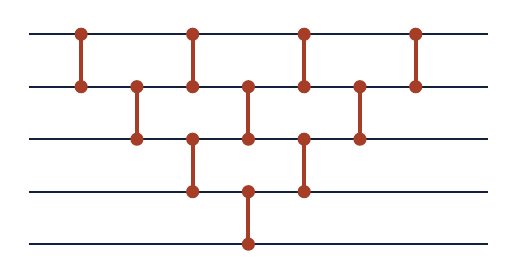
\begin{tikzpicture}[pxgrid]
  \foreach \y in {50,130,210,290,370} \draw[navy, line width=3\px] (30,\y) -- (730,\y);
  \begin{scope}[rust]
    \cmp{110}{50}{130} \cmp{195}{130}{210} \cmp{280}{210}{290} \cmp{280}{50}{130}
    \cmp{365}{290}{370} \cmp{365}{130}{210} \cmp{450}{210}{290} \cmp{450}{50}{130}
    \cmp{535}{130}{210} \cmp{620}{50}{130}
  \end{scope}
\end{tikzpicture}\par\vspace{0.15cm}
{\scriptsize\color{muted}Bubble sort on 5 wires: 10 comparators, but only 7 parallel layers ($2n-3$).}
\end{column}
\begin{column}{0.48\textwidth}
\textbf{Wires} carry items left to right.\par\medskip
\textbf{Comparators} put the smaller item on the upper wire and the larger on the lower one.\par\medskip
\textbf{Layers} are comparators on disjoint wires, run at the same time.\par\medskip
\textbf{Depth} is the number of layers. $D(n)$ is the least depth that sorts every input of size $n$.
\end{column}
\end{columns}
\note{0:40. Report Section 2 and Appendix G. This five-wire illustration has ten comparisons in seven layers. It is a simple example, not an optimal network. The zero-one principle justifies binary verification.}
\end{frame}

% ======================= 4. Batcher =======================
\begingroup\altstyle
\begin{frame}{Divide and conquer with an exact halving step}{Background \textperiodcentered\ Batcher's sort}
\begin{columns}[c]
\begin{column}{0.46\textwidth}
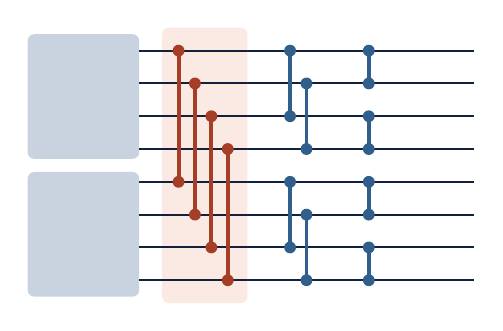
\begin{tikzpicture}[pxgrid]
  \fill[mist, rounded corners=10\px] (20,20) rectangle (190,210);
  \fill[mist, rounded corners=10\px] (20,230) rectangle (190,420);
  \fill[hl, rounded corners=10\px] (225,10) rectangle (355,430);
  \foreach \y in {45,95,145,195,245,295,345,395} \draw[navy, line width=3\px] (190,\y) -- (700,\y);
  \begin{scope}[rust]
    \cmp[9]{250}{45}{245} \cmp[9]{275}{95}{295} \cmp[9]{300}{145}{345} \cmp[9]{325}{195}{395}
  \end{scope}
  \begin{scope}[steel]
    \cmp[9]{420}{45}{145} \cmp[9]{445}{95}{195} \cmp[9]{420}{245}{345} \cmp[9]{445}{295}{395}
    \cmp[9]{540}{45}{95} \cmp[9]{540}{145}{195} \cmp[9]{540}{245}{295} \cmp[9]{540}{345}{395}
  \end{scope}
\end{tikzpicture}\par\vspace{0.1cm}
{\scriptsize\textcolor{steel}{\textbf{Grey:} sort halves}\quad \textcolor{rust}{\textbf{Red:} halving layer}\quad \textcolor{muted}{\textbf{Blue:} recurse}}
\end{column}
\begin{column}{0.50\textwidth}
\textbf{1.} Sort the two halves in parallel, one ascending and one descending.\par\medskip
\textbf{2.} One layer comparing wire $i$ with wire $i+n/2$ now \textbf{exactly halves} the items: every item on top is smaller than every item below.\par\medskip
\textbf{3.} Recurse on each half. Merging costs $\log_2 n$ layers, so sorting costs $\tfrac12\log_2 n\,(\log_2 n+1)$.
\end{column}
\end{columns}
\note{0:45. Report Appendix G. This is Batcher bitonic sorting on a power-of-two width. Sort halves in opposite directions before applying the exact split. The recursive merge costs log2 n layers, and the sorter has triangular depth.}
\end{frame}
\endgroup

% ======================= 5. epsilon-halver =======================
\begin{frame}{AKS halves cheaply and corrects the errors}{Background \textperiodcentered\ The AKS idea}
\begin{columns}[c]
\begin{column}{0.42\textwidth}
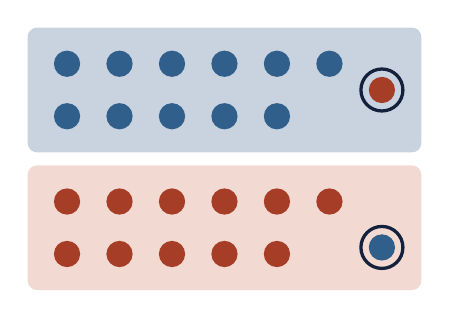
\begin{tikzpicture}[pxgrid]
  \fill[mist, rounded corners=14\px] (20,20) rectangle (620,210);
  \fill[softrust, rounded corners=14\px] (20,230) rectangle (620,420);
  \foreach \x in {80,160,240,320,400,480} {\fill[steel] (\x,75) circle[radius=20\px]; \fill[rust] (\x,285) circle[radius=20\px];}
  \foreach \x in {80,160,240,320,400} {\fill[steel] (\x,155) circle[radius=20\px]; \fill[rust] (\x,365) circle[radius=20\px];}
  \fill[steel] (560,355) circle[radius=20\px]; \fill[rust] (560,115) circle[radius=20\px];
  \draw[navy, line width=5\px] (560,115) circle[radius=32\px] (560,355) circle[radius=32\px];
\end{tikzpicture}\par\vspace{0.1cm}
{\scriptsize\textcolor{steel}{\textbf{Blue:} small items}\quad \textcolor{rust}{\textbf{Red:} large items}\quad \textcolor{muted}{\textbf{Circled:} misplaced}}
\end{column}
\begin{column}{0.54\textwidth}
\textbf{$\varepsilon$-halver:} for $k\le n/2$, of the $k$ smallest items, at most $\varepsilon k$ end up in the bottom half (and likewise for the largest).\par\medskip
\textbf{Constant depth:} built from a few matchings of an expander graph, independent of $n$.\par\medskip
\textbf{The catch:} halving and recursing lets errors pile up. AKS keeps a tree of bags and sends items that look out of place \textbf{back up} to be re-sorted.
\end{column}
\end{columns}
\note{0:50. Report Appendix G. For fixed epsilon, a halver has constant depth. The rank guarantee is for each k at most n/2, on both sides. Recursion alone does not repair items sent into the wrong subtree.}
\end{frame}

% ======================= 6. Expander =======================
\begingroup\altstyle
\begin{frame}{A bipartite expander gives a constant-depth halver}{Background \textperiodcentered\ Building an $\varepsilon$-halver}
\begin{columns}[c]
\begin{column}{0.42\textwidth}
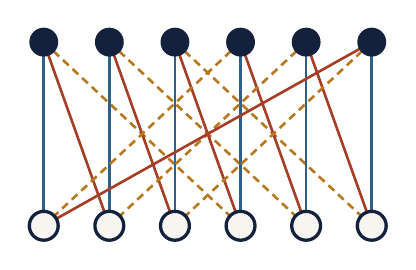
\begin{tikzpicture}[pxgrid]
  \foreach \i in {0,...,5} {
    \pgfmathtruncatemacro{\a}{mod(\i+1,6)} \pgfmathtruncatemacro{\b}{mod(\i+3,6)}
    \draw[steel, line width=4\px] (70+100*\i,80) -- (70+100*\i,360);
    \draw[rust, line width=4\px] (70+100*\i,80) -- (70+100*\a,360);
    \draw[amber, line width=4\px, dash pattern=on 12\px off 8\px] (70+100*\i,80) -- (70+100*\b,360);
  }
  \foreach \i in {0,...,5} {
    \fill[navy] (70+100*\i,80) circle[radius=22\px];
    \draw[navy, fill=paper, line width=5\px] (70+100*\i,360) circle[radius=22\px];
  }
\end{tikzpicture}\par\vspace{0.1cm}
{\scriptsize\textbf{Top row:} top-half wires\quad \textbf{Bottom row:} bottom-half wires\par}
{\tiny\color{muted}Each colour is one matching and one layer. This diagram is schematic, not a certified expander.\par}
\end{column}
\begin{column}{0.54\textwidth}
\textbf{1. Layers.} A $d$-regular bipartite graph between the halves splits into $d$ perfect matchings (Hall's theorem). Each becomes one layer.\par\medskip
\textbf{2. Stuck wires.} In a binary input, a top wire ending in 1 always held 1. Every bottom neighbour then ends in 1 too.\par\medskip
\textbf{3. Expansion.} If too many large items stay on top, their neighbours would require more large items than exist. Suitable expansion gives the halver guarantee.
\end{column}
\end{columns}
\note{0:50. Report Appendix G. The drawing only illustrates three matchings. It is not claimed to certify an epsilon-halver. In a binary run, a top wire ending in one always held one, and each neighbour on the bottom ends in one. The stuck set and its neighbourhood cannot contain more ones than the input. Suitable expansion rules out a large stuck set. Credit the published AKS construction.}
\end{frame}
\endgroup

% ======================= 7. Landscape =======================
\begingroup\altstyle
\begin{frame}{The logarithmic-depth gap}{Background}
\small
\begin{tabular}{p{0.36\textwidth}p{0.30\textwidth}p{0.23\textwidth}}
\toprule
\textbf{Result} & \textbf{Depth} & \textbf{Comment}\\
\midrule
Batcher (1968) & $\tfrac12\log_2 n(\log_2 n+1)$ & Simple construction\\
\rowcolor{hl} Ajtai, Koml\'os, Szemer\'edi (1983) & $O(\log n)$ & Large constant\\
Chv\'atal (1992) & $1830\log_2 n-58657$ & $n\ge 2^{78}$\\
Exact values of $D(n)$ & Known through 17 wires & Prior work\\
First unresolved width & $10\le D(18)\le11$ & One-layer gap\\
\bottomrule
\end{tabular}\par\vspace{0.4cm}
{\color{navy}We seek simpler constructions and proofs that explain what forces another layer. The numerical small-width optima are prior work.}
\note{0:45. Report Section 1, Section 10.1 and Appendix G. These are prior results. The new numerical contribution concerns a parameter choice within Chvatal, discussed later. The first unresolved exact width in the cited catalogue is eighteen.}
\end{frame}
\endgroup

% ======================= 8. Purpose =======================
\begin{frame}{Use AI agents to understand shallow sorting networks better}{Purpose of this effort}
\begin{columns}[T]
\begin{column}{0.48\textwidth}
\begin{card}{AKS analysis}A simpler, clearer account of why the AKS network works\end{card}
\begin{card}{Lower bounds}Extract structural obstructions and give human-understandable proofs of known bounds\end{card}
\end{column}
\begin{column}{0.48\textwidth}
\begin{card}{New constructions}$O(\log n)$-depth networks that are simpler or connect to other mathematics\end{card}
\begin{card}{Fixed $n$}Find shallower sorting networks for specific values of $n$\end{card}
\end{column}
\end{columns}
\vspace{0.2cm}
{\scriptsize\color{muted}Claude and Codex: main research and writing. DeepSeek V4.1 Flash and KimiK3.1 Pro: initial analysis.}
\note{0:45. Report Sections 1, 8 and 11. The four directions are research objectives, not claims that all were achieved. SAT supplies examples and constraints; LLM-assisted analysis helps search for proofs. Model-specific contributions are not inferred solely from branch names.}
\end{frame}

% ======================= 9. Outcomes =======================
\begingroup\altstyle
\begin{frame}{Three concrete outcomes}{Statement of outcomes}
\begin{columns}[T]
\begin{column}{0.31\textwidth}
\begin{card}{Lower bounds}{\rmfamily\bfseries\large\color{navy}Raised known bounds\par}\smallskip
One recurrence, $D(n)\ge D(\lceil n/2\rceil)+2$, adds one or two layers to the catalogued lower bounds for 25 to 64 wires.\end{card}
\end{column}
\begin{column}{0.31\textwidth}
\begin{card}{AKS analysis}{\rmfamily\bfseries\large\color{navy}A smaller coefficient\par}\smallskip
A checked parameter choice gives coefficient $5236/3\approx1745.33$ within Chv\'atal's existing construction.\end{card}
\end{column}
\begin{column}{0.31\textwidth}
\begin{card}{Constructions}{\rmfamily\bfseries\large\color{navy}Concrete shallow networks\par}\smallskip
Verified depths 26, 34, 43 and 52 at 128, 256, 512 and 1024 wires. These improve the Batcher baseline.\end{card}
\end{column}
\end{columns}
\vspace{0.3cm}
{\color{muted}A simpler logarithmic-depth construction remains an objective.}
\note{1:00. Report Sections 1, 2, 9 and 10.1. Separate the raised lower bounds, the explicit parameter theorem, and verified finite constructions. The bounds for 25 to 64 wires improve on those listed in Dobbelaere's catalogue (checked 15 November 2026); priority in the wider literature is not established. The small-width optimal depths and the AKS architecture are prior work. A simpler logarithmic-depth architecture remains open.}
\end{frame}
\endgroup

% ======================= 10. Halving lemma statement =======================
\begingroup\darkstyle
\begin{frame}{The halving lemma}{Outcome 1 \textperiodcentered\ Lower bounds for small $n$}
\vspace{0.35cm}
{\color{paper}\fontsize{32}{36}\selectfont $D(n)\;\ge\; D(\lceil n/2\rceil)+2$\par}
\vspace{0.45cm}
{\Large\color{mist}For $n\ge3$, sorting $n$ items needs at least two more layers than sorting half of them.\par}
\vspace{0.4cm}
{\color{rustlight}The two-layer removal and this recurrence are verified in Lean.}
\note{1:00. Report Section 2.1 and Appendix E.4. The hypothesis n at least three matters. For n=2 the formula is false. Lean checks only the two-layer removal and halving recurrence, not all the report theorems. Larger consequences can use published small-width depths, but those are separate premises.}
\end{frame}
\endgroup

% ======================= 11. Halving proof =======================
\begin{frame}{Freeze half the wires for two layers}{Outcome 1 \textperiodcentered\ Proof idea}
\begin{columns}[c]
\begin{column}{0.46\textwidth}
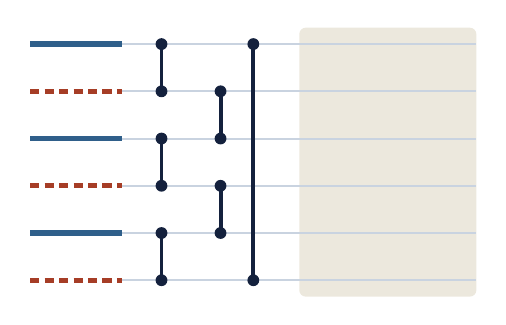
\begin{tikzpicture}[pxgrid]
  \fill[paperalt, rounded corners=10\px] (430,15) rectangle (700,425);
  \foreach \y in {40,112,184,256,328,400} \draw[mist, line width=3\px] (160,\y) -- (700,\y);
  \foreach \y in {40,184,328} \draw[steel, line width=8\px] (20,\y) -- (160,\y);
  \foreach \y in {112,256,400} \draw[rust, line width=8\px, dash pattern=on 14\px off 8\px] (20,\y) -- (160,\y);
  \begin{scope}[navy]
    \cmp[9]{220}{40}{112} \cmp[9]{220}{184}{256} \cmp[9]{220}{328}{400}
    \cmp[9]{310}{112}{184} \cmp[9]{310}{256}{328} \cmp[9]{360}{40}{400}
  \end{scope}
\end{tikzpicture}\par\vspace{0.1cm}
{\scriptsize\textcolor{steel}{\textbf{Solid:} variables}\quad \textcolor{rust}{\textbf{Dashed:} $\pm\infty$ constants}\quad \textcolor{muted}{\textbf{Shaded:} later layers}}
\end{column}
\begin{column}{0.50\textwidth}
\textbf{1.} Fill the first layer if needed. The first two layers form paths and even cycles, so their graph is 2-colourable.\par\medskip
\textbf{2.} Put $\pm\infty$ on one colour class, choosing signs that stay fixed in layer 1. No two variables meet in layers 1--2.\par\medskip
\textbf{3.} Follow the $\ge n/2$ variables as tokens. Layers $3,\dots,d$ sort them, and Knuth's untangling turns this into a real sorter of depth $d-2$.
\end{column}
\end{columns}
\note{1:10. Report Section 2, Theorem 2.1. First fill the first layer without increasing depth. Its union with the next layer consists of paths and even cycles. Select one colour class and sign the sentinels to remain stationary during the first layer. Both layers are blind. Follow the real values and untangle to obtain a sorter on the surviving inputs.}
\end{frame}

% ======================= 12. Small bounds =======================
\begingroup\altstyle
\begin{frame}{Hand proofs through ten wires}{Outcome 1 \textperiodcentered\ Consequences}
\begin{columns}[T]
\begin{column}{0.52\textwidth}
\begin{tabular}{cc}
\toprule
\textbf{Wires $n$} & \textbf{Optimal depth $D(n)$}\\
\midrule
1 & 0\\
2 & 1\\
3--4 & 3\\
5--6 & 5\\
7--8 & 6\\
\rowcolor{hl}9--10 & 7\\
\bottomrule
\end{tabular}\par\vspace{0.2cm}
{\scriptsize\color{muted}Restrictions, a five-wire obstruction and monotonicity. Known constructions meet every lower bound.}
\end{column}
\begin{column}{0.44\textwidth}
\begin{card}{What changed}We now have a complete chain of hand arguments through ten wires, without SAT or computer-found size bounds as premises.\end{card}
\begin{caveat}The values were already known. For larger widths, the recurrence gives $D(32)\ge11$ using the published $D(16)=9$. We do not claim priority for that consequence.\end{caveat}
\end{column}
\end{columns}
\note{1:10. Report Section 2, Corollary 2.2, and Appendix A. Our starting point lacked a complete human proof of these small lower bounds. The seven-wire case uses a five-wire thin-layer obstruction; the nine-wire case follows from the recurrence. Known constructions provide the upper bounds. The D(32) consequence depends on the published D(16)=9 and has no priority claim.}
\end{frame}
\endgroup

% ======================= Current published lower bounds =======================
\begin{frame}{Published depth bounds: the starting point}{Outcome 1 \textperiodcentered\ Current catalogue}
\begin{columns}[T]
\begin{column}{0.53\textwidth}
\begin{tabular}{ccc}
\toprule
\textbf{Wires $n$} & \textbf{Lower bound} & \textbf{Status}\\
\midrule
11--12 & 8 & Exact\\
13--16 & 9 & Exact\\
17 & 10 & Exact\\
18--20 & 10 & Upper bound 11\\
21--24 & 10 & Upper bound 12\\
25--28 & 10 & Upper bound 13\\
29--32 & 10 & Upper bound 14\\
\bottomrule
\end{tabular}
\end{column}
\begin{column}{0.43\textwidth}
\begin{card}{Published optimality results}
Bundala--Z\'avodn\'y (BZ14) establish the depths for 11--16 wires. Codish et al.\ (CCEMS16) establish the 17-wire optimum.
\end{card}
\begin{caveat}
At 18 wires, $10\le D(18)\le11$ remains open. Our selected-prefix exclusions do not prove $D(18)\ge11$.
\end{caveat}
\end{column}
\end{columns}
\vspace{0.25cm}
{\scriptsize\color{muted}Source: \href{https://bertdobbelaere.github.io/sorting_networks.html\#BZ14}{Bert Dobbelaere's sorting-network catalogue, including BZ14 and CCEMS16}. Checked 15 November 2026. Depth counts layers, not comparators.}
\note{0:45. Published baseline from the linked catalogue, checked 15 November 2026. BZ14 is Bundala and Zavodny, Optimal sorting networks, LATA 2014. CCEMS16 is Codish, Cruz-Filipe, Ehlers, Muller and Schneider-Kamp, Sorting networks: To the end and back again, 2016. Exact means matching upper and lower depth bounds, independently of size optimality. Our small-width hand proofs recover known values. The first open width is 18. Report Section 1 supplies the published premises and the unresolved D(18) interval.}
\end{frame}

% ======================= Lower bounds from our transfer theorem =======================
\begingroup\altstyle
\begin{frame}{Our transfer theorem raises the listed lower bounds}{Outcome 1 \textperiodcentered\ New consequences}
\begin{columns}[T]
\begin{column}{0.51\textwidth}
\begin{tabular}{cccc}
\toprule
\textbf{Wires $n$} & \textbf{Catalogue} & \textbf{Ours} & \textbf{Gain}\\
\midrule
\rowcolor{hl}25--32 & 10 & \textbf{11} & +1\\
33--38 & 10 & \textbf{12} & +2\\
39--48 & 11 & \textbf{12} & +1\\
49--54 & 11 & \textbf{13} & +2\\
55--64 & 12 & \textbf{13} & +1\\
\bottomrule
\end{tabular}\par\vspace{0.2cm}
{\scriptsize\color{muted}All entries are lower bounds on $D(n)$; they do not establish optimal depths.}
\end{column}
\begin{column}{0.45\textwidth}
\begin{card}[rust]{One recurrence, three intervals}
$D(n)\ge D(\lceil n/2\rceil)+2$ for $n\ge3$.\par\smallskip
$D(13)=9\ \Rightarrow\ D(25\text{--}32)\ge11$.\par\smallskip
$D(17)=10\ \Rightarrow\ D(33\text{--}48)\ge12$.\par\smallskip
Apply it again: $D(49\text{--}64)\ge13$.
\end{card}
\begin{caveat}
These consequences use published small-width optima. They improve the catalogue's listed bounds; priority in the wider literature is not established.
\end{caveat}
\end{column}
\end{columns}
\vspace{0.2cm}
{\scriptsize\color{muted}Our result: report, Corollary 2.2. Baseline: \href{https://bertdobbelaere.github.io/sorting_networks.html}{Dobbelaere, up to 32 wires} and \href{https://bertdobbelaere.github.io/sorting_networks_extended.html}{extended catalogue, up to 64 wires}; checked 15 November 2026.}
\note{1:00. Report Section 2, Corollary 2.2. By monotonicity, widths 25 through 32 halve to at least 13, giving 9+2=11. Widths 33 through 48 halve to at least 17, giving 10+2=12. Widths 49 through 64 halve to 25 through 32, giving 11+2=13. The catalogue lists 10 through width 38, 11 at widths 39 through 54, and 12 at widths 55 through 64. These are improvements over that table, not a claim of first discovery across the literature. In particular, 11 <= D(32) <= 14 follows; D(32)=11 and D(32)>=12 do not.}
\end{frame}
\endgroup

% ======================= 12b. How the halving lemma was found =======================
\begin{frame}{Five questions led to the halving lemma}{Outcome 1 \textperiodcentered\ How it was found}
\small
\begin{enumerate}\setlength{\itemsep}{3pt}
\item {\color{navy}\textbf{Can $D(9)\ge7$ be proved by hand?}}\asker{Team}\\
Our starting proofs used computer-found sizes, $S(7)=16$ and $S(9)=25$.
\item {\color{navy}\textbf{What if $\pm\infty$ inputs go on any wires, not just at the ends?}}\asker[rust]{Claude}\\
Their paths are fixed in advance, so the network must still sort the remaining inputs.
\item {\color{navy}\textbf{Does $S(5)=9$ have a hand proof?}}\asker{Team}\\
Our first reduction, from 7 wires to 5, leaned on it. It became a premise to remove.
\item {\color{navy}\textbf{What if every first-layer comparator holds one infinity?}}\asker[rust]{Claude}\\
No two variables meet in layer 1. A search tried all 16 sign choices on 9 wires.
\item {\color{navy}\textbf{Why did that search stop at layer 2?}}\asker[rust]{Claude}\\
For every second layer, some sign choice kept the variables apart there too. The reason: layers 1--2 form paths and even cycles, so they can always be 2-coloured.
\end{enumerate}
\vspace{0.15cm}
\begin{statement}
The search was built to use $S(5)=9$, but it stopped for a reason that needs only $D(5)\ge5$. Explaining that reason gave the halving lemma.
\end{statement}
\note{0:50. Source: the Claude session log for the D(9) hand proof; this account is not yet in the report. A team member asked for a hand proof of D(9) at least 7, adding that even D(7) at least 6 might lack one. Claude placed infinities on interior wires, and the team member asked whether S(5)=9 has a hand proof, because the seven-to-five step used it. With one infinity in every first-layer comparator, a nine-wire search over sixteen sign choices was meant to prune with S(5)=9 counting. No second layer survived, for a reason that needs only D(5) at least 5. Explaining it gave the two-colouring, which was checked for every second layer up to eleven wires about half an hour after the first question.}
\end{frame}

% ======================= 13. Structural proofs =======================
\begin{frame}{Mining structural proofs from SAT}{Outcome 1 \textperiodcentered\ Pushing further}
SAT identifies constrained cases. We use LLM-assisted analysis to look for a reason that a human can check.\par\vspace{0.3cm}
\begin{columns}[T]
\begin{column}{0.31\textwidth}\begin{card}{A short proof}Two moving infinity restrictions force a nine-wire cycle case into a small family. Nine explicit rows finish the contradiction.\end{card}\end{column}
\begin{column}{0.31\textwidth}\begin{card}{Reusable structure}Merger arguments force a large interaction component. The nine-wire profile lemma now has hand coverage of 26 out of 50 classes.\end{card}\end{column}
\begin{column}{0.31\textwidth}\begin{card}[rust]{Current limit}At 18 wires we exclude selected longer prefixes, but none of the 411 complete two-layer cases is closed.\end{card}\end{column}
\end{columns}
\vspace{0.3cm}
{\color{navy}The goal is a structural theorem that reaches beyond large case searches.}
\note{1:20. Report Sections 6 and 7, Appendix F. In the nine-wire cycle case, opposite-sign sentinel placements remain disjoint, so their six-real sets always overlap in three wires. A matching cannot pair both sets internally. This forces a small family, eliminated by nine rows. Full H9 still has computational dependencies in 24 classes. Selected D18 prefix exclusions do not close any of the 411 full two-layer cases.}
\end{frame}

% ======================= 15. Constants =======================
\begingroup\altstyle
\begin{frame}{Comparing constants in the same units}{Outcome 2 \textperiodcentered\ Constants}
\begin{columns}[T]
\begin{column}{0.54\textwidth}
\small
\begin{tabular}{ll}
\toprule
\textbf{Construction or proposal} & \textbf{Coefficient of $\log_2 n$}\\
\midrule
Chv\'atal (1992) & $1830$\\
\rowcolor{hl} New parameter choice & $5236/3\approx1745.33$\\
Seiferas, sample parameters & $\approx514{,}247$\\
Corrected Seiferas proposal & $\approx281{,}084$\\
Refined bookkeeping proposal & $\approx6300$\\
\bottomrule
\end{tabular}\par\vspace{0.2cm}
{\scriptsize\color{muted}All coefficients count comparator layers. The last two proposals remain unverified.}
\end{column}
\begin{column}{0.42\textwidth}
\begin{card}[rust]{New checked parameter bound}
$D(n)\le\frac{5236}{3}\log_2 n-40651$\par\smallskip
for $n\ge2^{79}$. The leading coefficient is about 4.63\% below Chv\'atal's.\end{card}
\begin{caveat}The full bound improves his only above $\log_2 n\approx212.67$. It uses the existing AKS construction and is not yet formalized in Lean.\end{caveat}
\end{column}
\end{columns}
\note{1:20. Report Section 10.1, Theorem 10.1, and Section 10.2. The new leading coefficient is about 4.63 percent smaller than 1830. Its larger additive offset means the complete affine bound improves Chvatal only for log2 n greater than 27009/127. Exact parameter inequalities and five stopping residues passed. This does not certify the older Seiferas proposals, prove a globally best constant, or replace the existing AKS architecture. Primary source: \url{https://doi.org/10.7282/T379487B}.}
\end{frame}
\endgroup

% ======================= 17. Depths =======================
\begin{frame}{Concrete constructions below the Batcher baseline}{Outcome 3 \textperiodcentered\ Results}
\begin{tabular}{p{0.11\textwidth}p{0.15\textwidth}p{0.17\textwidth}p{0.11\textwidth}p{0.26\textwidth}}
\toprule
$n$ & \textbf{Batcher} & \textbf{Lee--Batcher} & \textbf{Ours} & \textbf{Built from}\\
\midrule
\rowcolor{hl} 128 & 28 & 27 & \textbf{26} & $8\times 16$, then merge\\
256 & 36 & 34 & 34 & $2\times 128$, then merge\\
512 & 45 & 43 & 43 & $2\times 256$, then merge\\
\rowcolor{hl} 1024 & 55 & 53 & \textbf{52} & $8\times 128$, then merge\\
\bottomrule
\end{tabular}\par\vspace{0.4cm}
The Lee--Batcher column is the collaborator's evaluation of their formula. The multiway recursion is prior work. Priority against the full literature has not been established.
\note{0:55. Report Section 9, Table 2. The networks are verified upper bounds, not optimal depths. The Lee-Batcher values are the collaborator formula comparison, not a complete literature search. Do not call these globally best-known depths.}
\end{frame}

% ======================= 18. Verification =======================
\begingroup\altstyle
\begin{frame}{How we know the networks sort}{Outcome 3 \textperiodcentered\ Verification}
Checking all $2^{1024}$ zero-one inputs is impossible. Instead, an independent checker reads only the list of layers, rediscovers the structure, and checks each piece on every input that piece can receive.\par\vspace{0.3cm}
\begin{columns}[T]
\begin{column}{0.31\textwidth}\begin{card}{16-wire blocks}All $2^{16}$ inputs\end{card}\end{column}
\begin{column}{0.31\textwidth}\begin{card}{Base mergers}All $3^8$ inputs of 8 sorted pairs\end{card}\end{column}
\begin{column}{0.31\textwidth}\begin{card}{Cleanup layers}Every input they can receive, by induction\end{card}\end{column}
\end{columns}
\vspace{0.3cm}
\begin{columns}[T]
\begin{column}{0.48\textwidth}\textbf{Earlier controls, not rerun here:} all 6 networks with one comparator removed were rejected.\end{column}
\begin{column}{0.48\textwidth}\textbf{Earlier cross-check, not rerun here:} the 128-wire merger passed all $17^8$ sorted-block inputs.\end{column}
\end{columns}
\note{1:00. Report Section 9.1. The fresh compositional checks cover every comparator at all four widths. The 1024-wire network has 64 base sorters, 128 pair mergers and 119 cleanup steps. The extra deletion tests and 17^8-input merger test are historical checks recorded by the collaborator, not rerun for this synthesis.}
\end{frame}
\endgroup

% ======================= 19. Negative results =======================
\begin{frame}{What did not work, and why}{Other attempts}
\begin{columns}[T]
    \begin{column}{0.31\textwidth}\begin{card}{Simpler AKS Proof}{\rmfamily\bfseries\large\color{navy}We attempted to get a simpler proof that an AKS-style sorting network was correct, but we were not able to.}\end{card}\end{column}
    \begin{column}{0.31\textwidth}\begin{card}{Deleting a third layer}{\rmfamily\bfseries\large\color{navy}We were unable to find stronger structural constraints by considering the first three layers at once.} \end{card}\end{column}
    \begin{column}{0.31\textwidth}\begin{card}{Exact search}{\rmfamily\bfseries\large\color{navy}Improvements to $D(n)$ for $32 \ge n \ge 18$ failed due to the large search space that AI agents could not cut down.}\end{card}\end{column}
\end{columns}
\end{frame}

% ======================= 21. Open problems =======================
\begingroup\darkstyle
\begin{frame}{Where to go next}{Open problems}
\begin{enumerate}\setlength{\itemsep}{10pt}
\color{mist}
\item Extract a short invariant from SAT certificates and complete the remaining nine-wire hand cases.
\item Extend the structural arguments across complete prefix families, toward resolving $D(18)$.
\item Find a simpler logarithmic-depth construction or a clearer AKS proof with a smaller explicit constant.
\item Formalize all of our work in Lean, including the mathematics behind the computational certificates.
\end{enumerate}
\note{0:50. Report Sections 1 and 8, Appendix E.4. The formalization plan covers all mathematical results and the semantic justification of computational evidence. This is a future objective. Thank the audience and invite questions.}
\end{frame}
\endgroup

\end{document}
